\section{Materials}
\label{sec:materials}

The methods presented in this paper were devised as part of the development of
a larger software toolbox for fully automatic analysis of very-high-resolution
SRµCT bone tomograms. Presently, the work is focused on the automatic analysis
of an experiment conducted to evaluate four different methodologies for
stimulating bone regeneration in goat mandibles, described below. The software
system is also being developed as preparatory work for the analysis of SRµCT
bone tomograms from 150 human patients in the MAXIBONE project
% TODO (James): issue #10 1.39 ift at snakke evaluering af brugen af metode
% mht knogle m.v enten skal denne forward-reference, ellers skal den senere
% backward-reference.
(\url{www.maxibone.eu}). This project aims to create personalized maxillary
bone regeneration by using culture-expanded autologous bone marrow stem cells
and biomaterials, for which clinical trials are presently being conducted. The
data set used in the present work is 35 high-resolution tomograms of old and
regenerated goat mandible bone samples, to evaluate the amount and health of
regenerated bone, and in particular, zooming in on osseointegration against the
titanium implants closer than was previously done.

\subsection{Background for the medical experiment} Installation of a dental
implant initiates the Regional Acceleratory Phenomenon (RAP), which implies an
acceleration of the different healing stages. RAP begins a few days after
implant installation, peaks at 1-2 months, and subsides after 6-24
months~\cite{frost1989}. In cortical bone, the non-vital mineralized tissue
initially needs to be resorbed prior to bone formation. In the cancellous
compartment, the implant installation mainly results in damage to marrow spaces
with resulting local bleeding and coagulum formation. The coagulum gradually
resorbs, collagen is laid down and replaced by osteoid, and eventually --- if
sufficient blood supply is present --- woven immature bone develops, and
sequentially osseointegration is initiated~\cite{frost1989}. After 6-12 weeks
of healing, most of the woven bone is mineralized and bone marrow containing
blood vessels, adipocytes, and mesenchymal cells can be observed surrounding
the trabeculae in the mineralized bone~\cite{Berglundh2003, Abrahamsson2004}. A
cement line, thickness of 0.2-5µm, will be deposited directly on the implant
surface during continuous bone formation. The biological fixation of the
implant initiates only a few days after implant installation, where the
osteoblasts begin to deposit collagen matrix on the cement line. This early
deposition of calcified matrix followed by the arrangement of woven bone and
later mature cancellous bone develops in a 3D manner delimiting the marrow
space~\cite{Franchi2004}.

\subsection{Physical samples}

The experiment evaluated four methods for stimulating maxillary bone
regeneration. 5 critical size defects were introduced to 7 goats. Four defects
were used to assess bone regeneration methods, and one was a control sample.
Peri-implant vertical bone augmentation was performed using autologous bone and
two different calcium phosphate bone substitutes. The bone specimens were
evaluated undecalcified. The specimen preparation was performed at the
Department of Biomaterials at Gothenburg University, Sweden. The specimens were
initially fixated in 4\% paraformaldehyde. Dehydration of the specimens was
performed in increasing concentrations of ethanol to eliminate fat and water
content. Furthermore, specimens were infiltrated with methylmethacrylate (MMA)
and embedded in molds 12 mm in diameter and 20 mm in
height~\cite{NELDAM2015682}. They were scanned at the European Synchrotron
Radiation Facility (ESRF) in Grenoble, France. The advantage of using MMA is
greater tissue penetration than water-soluble methacrylates. This is an
advantage when preparing larger specimens such as bone biopsies containing
dental implants. Furthermore, the histological quality of bone sections is
generally higher for MMA-embedded specimens compared to water-soluble
methacrylates~\cite{erben1997}. Additionally, tissue shrinkage is less than 2\%
when using MMA-embedded bone and cartilage specimens~\cite{ferguson1999}.

% TODO (James): shouldn't the 2.5 and 5.5 be swapped??? Also calling it upper and lower
% is redundant when not defining a direction... also 8mm is not possible!
% It more seems like 3+2mm=5mm for small/large threads respectively
% ... also the implant is 5.9 mm x 3.4 mm along largest dimensions
% - so while it is not too important to talk about how the samples were prepared, it
% definitely is important to know the dimensions of our cut samples
Physical samples were prepared for SRµCT scanning by cutting out portions from
the larger cylindrical biopsies. Within these samples, we find the titanium
dental implant (Astra Tech OsseoSpeed, ST Molndal, Sweden).  It is 3.5 mm in
diameter and 8 mm long. Along its length, the lower 5.5 mm has larger threads and
is attached to the recipient bone. The upper 2.5 mm has smaller threads and is
where the newly formed bone is to be assessed. Surrounding the bone and implant
contact region are cavities containing resin, air, blood vessels and other
fibrous tissue.

\begin{figure}
  \centering
  \begin{tabular}{cc}
    (a) & \begin{tabular}{c} 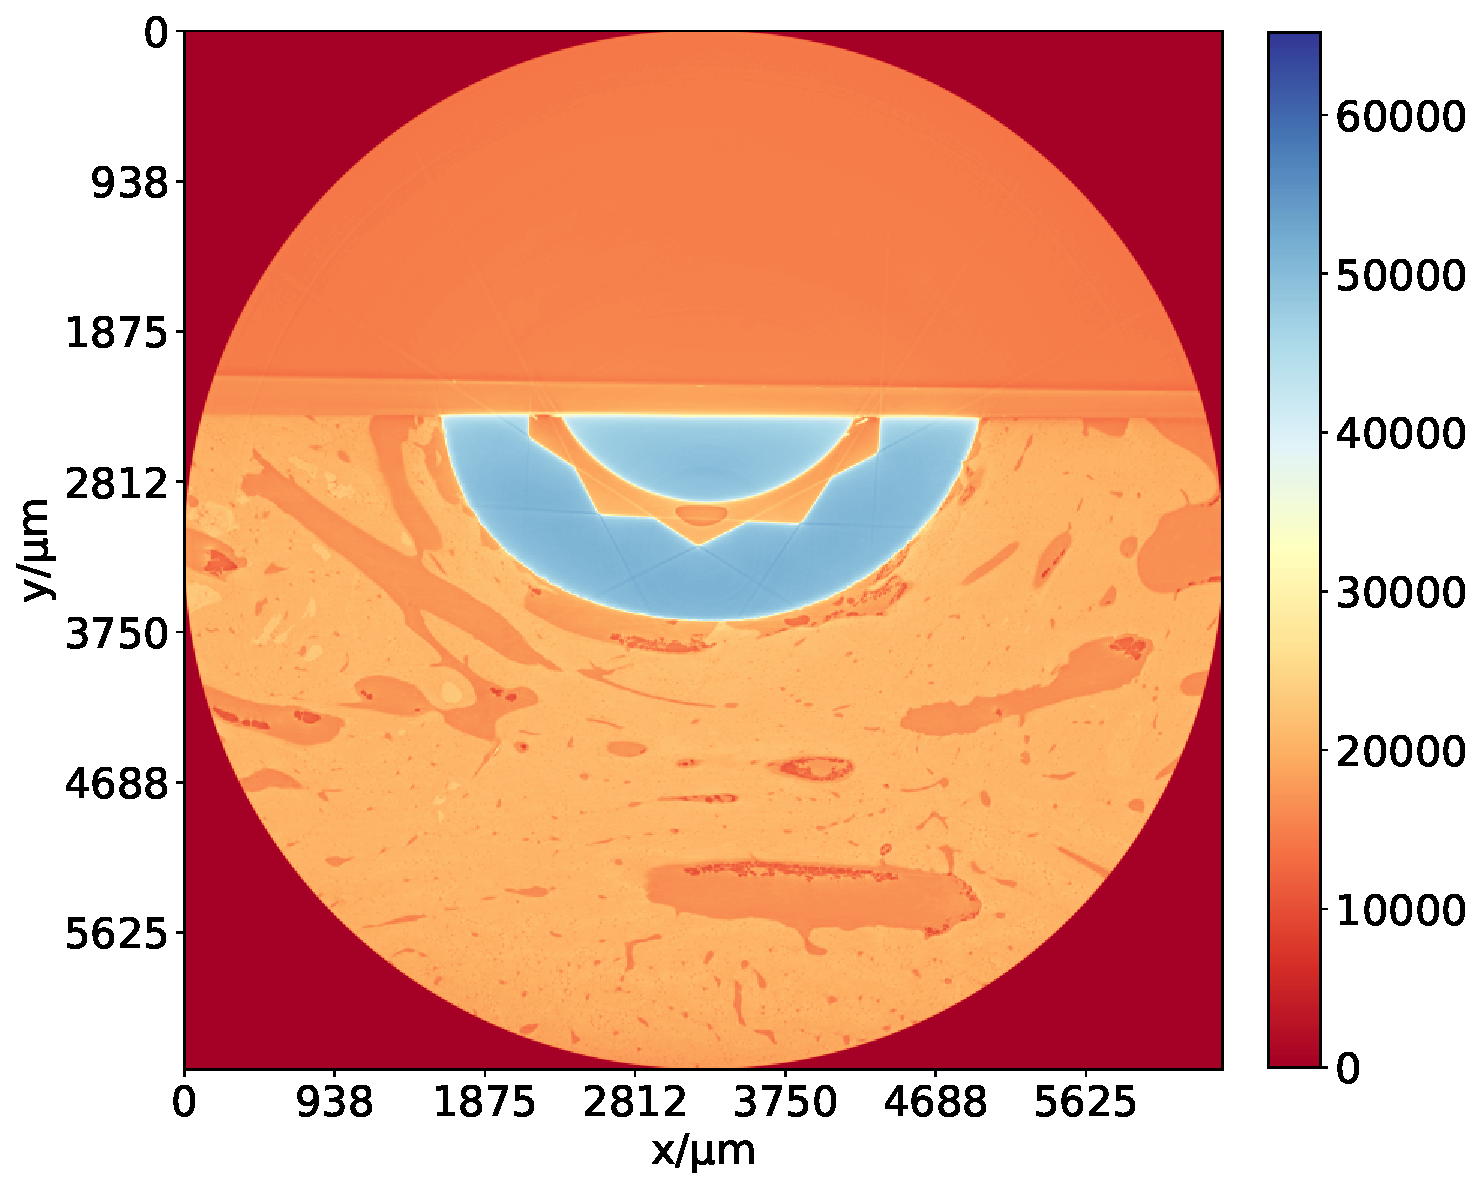
\includegraphics[width=0.81\linewidth]{generated/770c_pag_full_yx.pdf}\end{tabular}\\
    (b) & \begin{tabular}{c} 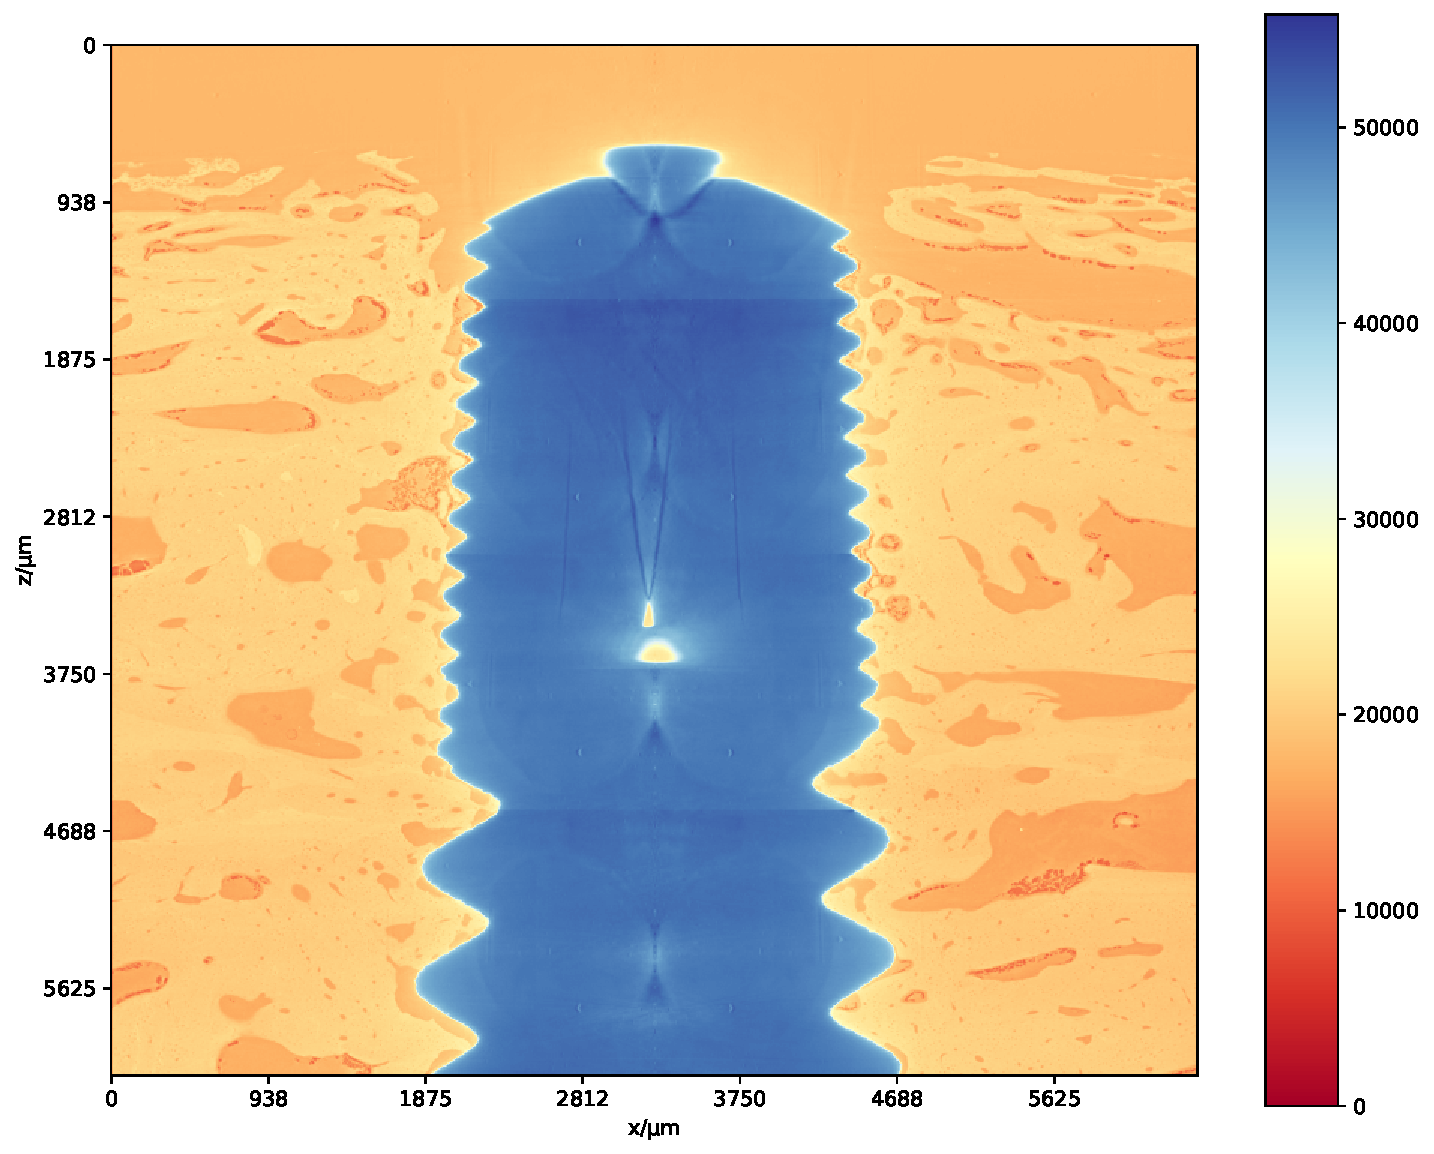
\includegraphics[width=0.81\linewidth]{generated/770c_pag_full_zx.pdf}\end{tabular}\\
    (c) & \begin{tabular}{c} 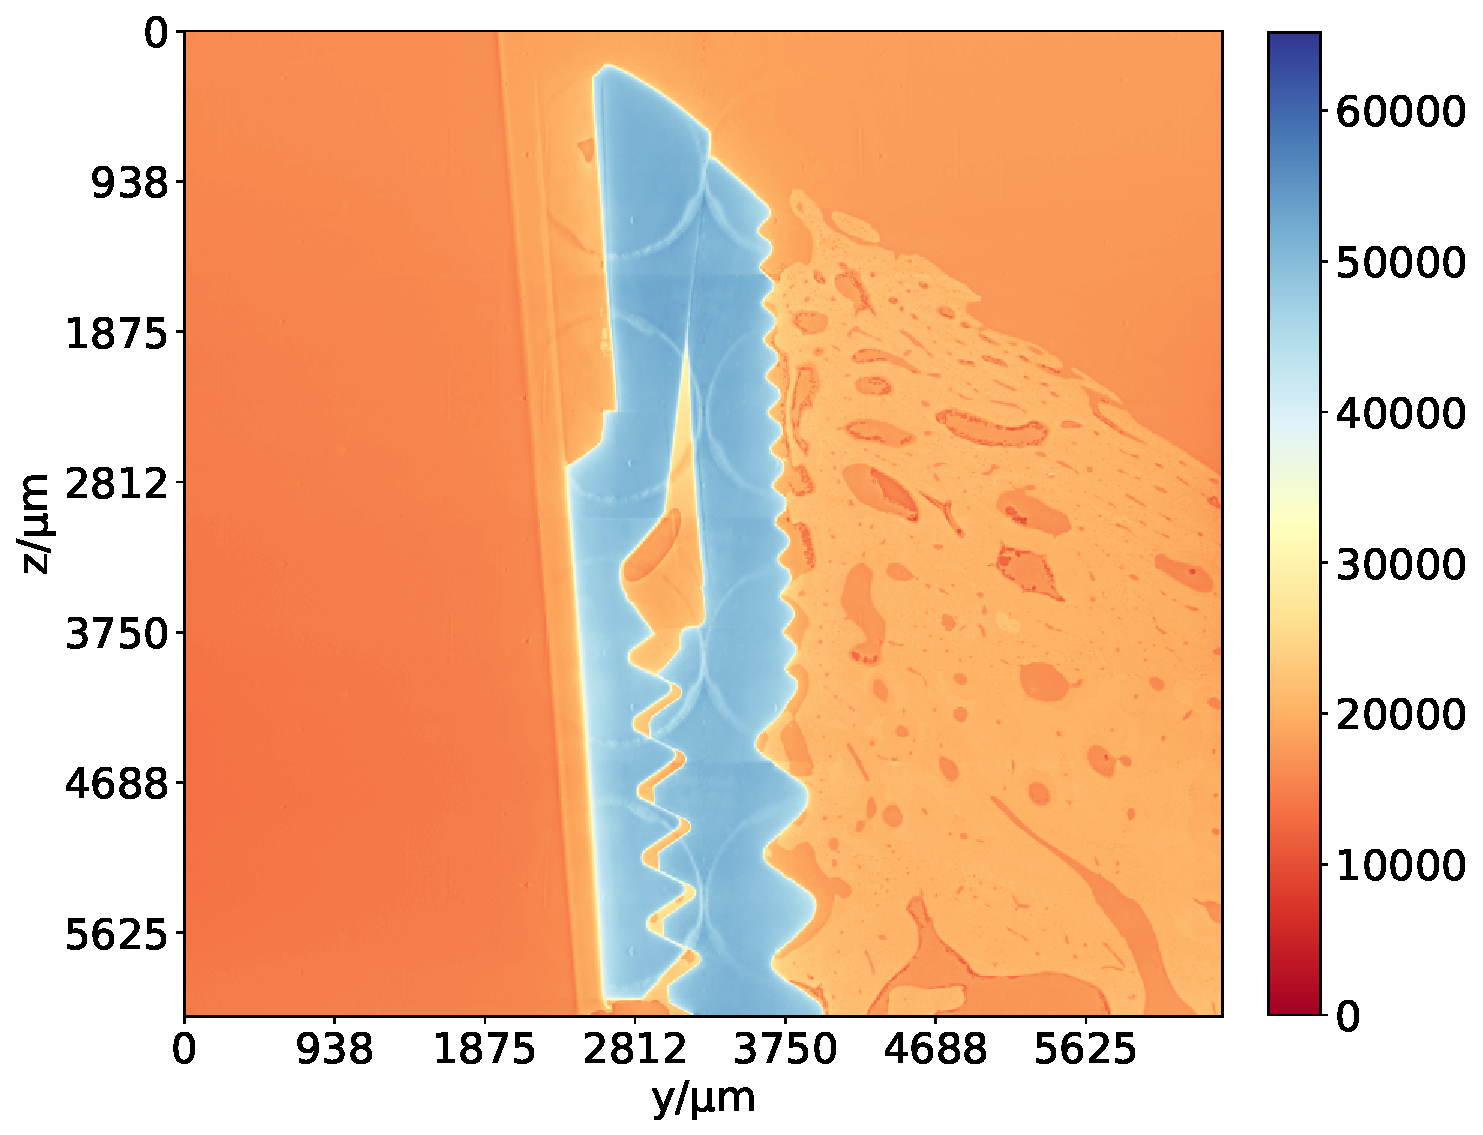
\includegraphics[width=0.81\linewidth]{generated/770c_pag_full_zy.pdf}\end{tabular}
  \end{tabular}
  \caption{
	The physical samples are scanned in chunks of 4-6 sub-volumes through
	the height of the implant, depending on the initial size of a sample.
	The physical field of view of a single image sample is about 6.5 mm in
	each direction. A voxel has a size of 1.875 µm.  Shown here are the
	cross sections of a reconstructed sample in the YX-, ZX- and ZY-planes
	respectively.
  }
\label{fig:3viewsample}
\end{figure}

A cut sample is shown in three different cross-sectional views in
\Cref{fig:3viewsample}. Each material has a unique density and thus absorption.
The titanium implant shown in blue has a higher absorption level than bone.
Bone material shown in light orange has higher absorption than its surrounding
dark orange-colored regions containing blood vessel tissue, air and resin.

\subsubsection{Data acquisition}

It can be difficult to study and evaluate the bone structure and blood network
without destroying or manipulating the sample. X-ray computed tomography is a
widely used tool for non-intrusive medical imaging. By exposing a subject to
X-rays, we can map the linear attenuation coefficient of the passing rays. Each
ray is attenuated relatively to the density and composition of the material it
passes. By rotating the sample we can reconstruct a 3D image representation of
the inner structure of the sample. Each volumetric pixel (voxel) then
represents the X-ray attenuation at its spatial position. In this way, X-rays
can reliably be used to internally characterize samples in a non-intrusive and
non-destructive manner. Medical CT scans can provide spatial resolutions on the
order of submillimetre scale \cite{medicalct}. The more modern micro-computed
tomography (µCT) can provide much higher spatial resolution on the micrometer
scale \cite{srexptime}.

This work focuses on data acquired by SRµCT.  Contrary to both CT and µCT, this
is not standard medical or laboratory equipment, but requires a large scale
particle accelerator facility.  For this imaging technique, electrons are
accelerated to ultra-relativistic speeds in trajectories directed by strong
magnetic fields. The resulting X-ray beam is narrow and of high photon flux
allowing faster scanning times \cite{srexptime}, making efficient use of the
beamtime and can also help counter Poisson noise from suboptimal photon count
\cite{srnoise}. Synchrotron radiation is high in brilliance and very well
collimated, allowing a better spatial resolution and a very high signal-to-noise
ratio.  Artifacts from beam-hardening are minimized due to synchrotron radiation
X-rays being characterized by their practically mono-energetic spectrum
\cite{srbeamquality}.

The tomograms in this work have been acquired at the ID19 beamline at the
European Synchrotron Radiation Facility (ESRF) in Grenoble, France. The
reconstruction~\cite{sporring} took place at the ID19 beamline, using the ESRF
in-house developed software PyHST~\cite{NELDAM2015682,pyhst}. PyHST was applied
with Paganin phase retrieval to improve reconstruction quality
~\cite{MIRONE201441}. All tomograms were acquired at 50 keV.

%%% Local Variables:
%%% mode: latex
%%% TeX-master: "main"
%%% End:
